\chapter{Evaluation}
\label{ch:evaluation}

This chapter presents results of number of experiments we have run. This includes 
We report on the feedback that is received from users' interaction through the use of the wePorter web interface. We show how it can be used for the purposes of filtering segments of interest within a video and the configuration of a new video story from the initially unstructured content. We present results from a user evaluation study on the merit of filtered and reconfigured content. We end with a reflection on our results in the discussion section.

\section{Setup}
For our experiments described in this section we use a set of 10 unedited, user-generated videos that were returned in response to a query for ``Diamond Jubilee London'' on YouTube. The videos along with their title and length is shown in table \ref{tab:videos}

\begin{table}
  \begin{center}
  \begin{tabular}{c}
    
  \end{tabular}
  \end{center}
  \caption{Videos used in the wePorter experiment}
  \label{label}
\end{table}

\section{Results}

\subsection{Preliminary Experiments} % (fold)
\label{sub:preliminary_experiments}

\subsubsection{Positional Bias}
Positioning two video's one on top of the other, might inflict a bias for users in their attentional behaviour. It might be the case that videos on the top are systematically more attended to than videos displayed below. We've experimented to see whether such positioning bias effects occur.

\subsubsection{Context Dependency}
We propose a statistical analysis of interaction data to inform the reconfiguration of initially unstructured video parts. We hypothesise that:
\begin{enumerate}
  % \item The perceived quality of a video reconfiguration is dependent on the sequential ordering of its internal parts
  \item Users' attentional behaviour depends on the sequential ordering of video parts
  \item Data about users' attentional behaviour can indicate what are preferred orderings.
\end{enumerate}

Before we investigate the second hypothesis in section \ref{sec:main_experiments}, we must scrutinise the first. In order to test whether users' attentional behaviour is dependent on the sequential ordering of video parts we have run a experiment in two trials. The first of these had 35 participants, the second 28. In each trial participants were presented with with a two sequences of three video parts playing back continuously using the parallel video player described in section \ref{sec:weporter_interface}. Based on random picks, roughly half of the participants were labelled as control group the others as test group. Participants in this group where shown two sequences where all video parts originated from different sources. This was changed for the second group, where participant were shown parts across the sequences that clearly belong to the same source video. 

The first trial presented test group users with a first part in the bottom sequence that was followed by a part from the same source video as the third part in the top video.

The second trial presented test group users with pieces from the same source video in the first and third part of the top sequence and second part of the bottom sequence.

The baseline sequences shown to control group participants had video parts of different sources on all positions and had final parts of both sequences identical to test group users.

A visual description of these conditions is shown in figure \ref{fig:exp_context}. Where we use the same conventions to display sequences, video parts and colouring to indicate source videos as in figure \ref{fig:framework}.

\begin{figure}[htbp]
  \centering
    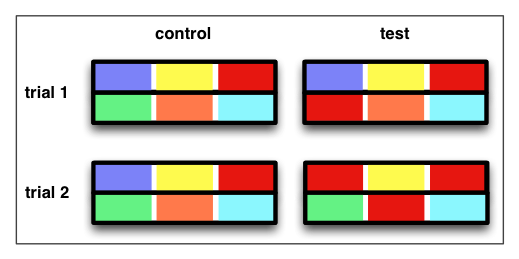
\includegraphics[width = .7\textwidth]{img/exp_context}
  \caption{Experimental Setup for Context Dependency}
  \label{fig:exp_context}
\end{figure}

% subsection preliminary_experiments (end)


\subsection{Clean Data} % (fold)
\label{sub:clean_data}

% subsection clean_data (end)


\section{Main Experiments} % (fold)
\label{sec:main_experiments}

% section main_experiments (end)


\subsection{Landscapes of Interest}

The distinction to be made, between interesting intervals on one hand and less striking parts of a video on the other is not likely to be a very strict one. Afterall, an unedited video captures a single stretch of space and time, so any event that is of particular interest will unlikely have hard cut-off points in time. Rather, if we see interest as a function of time in a particular video, we would expect a somewhat continuous flowing line with spikes every now and then when an interesting event occurs. 

Looking at interest at a more global level, aggregating over a large group of users, would perhaps even a more smooth landscape of interest. This kind of data could reveal mountains and valleys that can be used for interest-based segmentation. From the thus segmented parts, the ones with high interest scores can be returned as the salient parts within a video.

\section{Discussion}

\subsection{Feedback from Comments}

\begin{quote}
  ``[...]the technology may though have many uses like the crowd sourcing of video editing or the training of AI to mimic human audio visual focus and attention'' - Mia
\end{quote}

As part of the user feedback form that is presented during our interaction experiments, we gave participants the option to leave their comments. Thinking of potential of the interface, some people hit the nail right on the head.

Overall a number of salient points emerged from the comments:

\begin{itemize}
  \item \textbf{``I would like to see news this way''} - People were positive about the way video was presented in parallel while giving them the option to interact.
  \item \textbf{``I believe there was a bug''} - A number of people reported difficulties in the playback of videos. Most issues concerned a one or more video parts not immediately playing after the preceding one had finished. Apart from such glitches causing less clean data, this caused some users to be confused.
  \item \textbf{``The subject and content of the videos was uninteresting''} - Many people said they were not particularly interested in the topic of the presented videos. This meant that often they weren't drawn strongly to one video or the other and did not feel a strong reason to focus their 
  
\end{itemize}


Some participants offered useful ideas as to how they saw the project could be extended:

\begin{quote}
  ``Idea is great and project full of potential, in particular for big events which are well covered and allow multi-angle views of an action. It would be interesting to have information about the content producer displayed discretely on the player. That way the audience could vote on the quality of a source, and in time reward the owner for it's content, encouraging him to submit more videos in this system.'' - Marc
\end{quote}
